% !TEX TS-program = pdflatex
% !TEX encoding = UTF-8 Unicode

% This is a simple template for a LaTeX document using the "article" class.
% See "book", "report", "letter" for other types of document.

\documentclass[11pt]{article} % use larger type; default would be 10pt

\usepackage[utf8]{inputenc} % set input encoding (not needed with XeLaTeX)

%%% Examples of Article customizations
% These packages are optional, depending whether you want the features they provide.
% See the LaTeX Companion or other references for full information.

%%% PAGE DIMENSIONS
\usepackage{geometry} % to change the page dimensions
\geometry{a4paper} % or letterpaper (US) or a5paper or....
% \geometry{margin=2in} % for example, change the margins to 2 inches all round
% \geometry{landscape} % set up the page for landscape
%   read geometry.pdf for detailed page layout information

\usepackage{graphicx} % support the \includegraphics command and options

% \usepackage[parfill]{parskip} % Activate to begin paragraphs with an empty line rather than an indent

%%% PACKAGES
\usepackage{hyperref}
\usepackage{amsmath}
\usepackage{amssymb}
\usepackage{booktabs} % for much better looking tables
\usepackage{array} % for better arrays (eg matrices) in maths
\usepackage{paralist} % very flexible & customisable lists (eg. enumerate/itemize, etc.)
\usepackage{verbatim} % adds environment for commenting out blocks of text & for better verbatim
\usepackage{subfig} % make it possible to include more than one captioned figure/table in a single float
% These packages are all incorporated in the memoir class to one degree or another...

%%% HEADERS & FOOTERS
\usepackage{fancyhdr} % This should be set AFTER setting up the page geometry
\pagestyle{fancy} % options: empty , plain , fancy
\renewcommand{\headrulewidth}{0pt} % customise the layout...
\lhead{}\chead{}\rhead{}
\lfoot{}\cfoot{\thepage}\rfoot{}

%%% SECTION TITLE APPEARANCE
\usepackage{sectsty}
\allsectionsfont{\sffamily\mdseries\upshape} % (See the fntguide.pdf for font help)
% (This matches ConTeXt defaults)

%%% ToC (table of contents) APPEARANCE
\usepackage[nottoc,notlof,notlot]{tocbibind} % Put the bibliography in the ToC
\usepackage[titles,subfigure]{tocloft} % Alter the style of the Table of Contents
\renewcommand{\cftsecfont}{\rmfamily\mdseries\upshape}
\renewcommand{\cftsecpagefont}{\rmfamily\mdseries\upshape} % No bold!

%%% END Article customizations

%%% The "real" document content comes below...

\title{A Method for Detecting Convergence of Machine Learning Algorithms with Cauchy-Style Estimates}
\author{Galen Novello}
%\date{} % Activate to display a given date or no date (if empty),
         % otherwise the current date is printed 

\begin{document}
\maketitle

\begin{abstract}
In this paper I propose a method for detecting the convergence of the method of learning algorithms with "Cauchy 
style" estimates.  Brief overviews of background information including  Cauchy sequences and various learning algorithms are provided.  As an explicit example, the method is applied to the convergence of gradient descent, the method of max DJ is presented and it is conjectured that this learning algorithm has converged on iteration $k$ if $\sum_{p=k-2n}^{k} \left( \max_{i \in \{0, \dots , n\}} |DJ_{i_{p}}| \right)\  <\ 1 $. Empirical evidenceleading to this conjecture is presented. It is shown how the method of max DJ is then applied to learning algorithms whose solutions must be minimized over non-convex sets and this extension is applied to a neural network. 

\end{abstract}

\section{Cauchy Sequences}
Cauchy Sequences are a well known tool for analyzing convergence of sequences.  Most people first encounter them in the context of real numbers
in an introductory course on real analysis or topology but the equivalence of being a Cauchy Sequence and being a convergent sequence is so important 
that it gets its own name and we call a topological space with such an equivalence complete.  You can find rather exotic examples of complete spaces in
the literature, but for the purposes of this conversation it will suffice to point out that closed metric spaces, and in particular $\mathbb{R}^{n}$, are complete.

A sequence $\theta_{i}$ is said to be a Cauchy sequence if for any $\epsilon > 0$ there is some $N$ for which $|\theta_{i} - \theta_{j}| < \epsilon$ for all $i, j > N$. 
The idea of this paper is to adjust this definition in two ways to create a method to detect the convergence of the coefficients of gradient descent 

\begin{itemize} 
\item By changing the condition ``for all $i,j > N$"  to
``for all $i$ such that $k - k_{0} < i < k$ " where $k$ is the index of the most recent iteration and $k_{0}$ is a ``window size" that depends on the number of variables in the model.  
\item By finding a bound on $\epsilon$ that will ensure (at least a high probability of) convergence of the model.  

\end{itemize}

\section{ApplyingThe Method to Gradient Descent}

\subsection{Gradient Descent}
The method of gradient descent is a regression algorithm that works to minimize a cost function by using 
the gradient to iteratively adjust the model. A good introduction to the method as well as an outline of it's justification 
can be found in \href{http://openclassroom.stanford.edu/MainFolder/CoursePage.php?course=MachineLearning}{open source resources from Andrew Ng's Machine Learning Course}, 
and it was these materials which guided me to creating the gradient descent algoritm used in this paper. 

To produce a model for quantity of interest $y$  as a function of variables 
$x_{1}, ... , x_{n}$ the method seeks coefficents $\theta_{0}, \theta_{1}, ... , \theta_{n}$ of the line 
$$y = \theta_{0} + \theta_{1} x_{1} + ... + \theta_{n} x_{n}.$$  
The error of a model $\Theta = (\theta_{0}, \theta_{1}, \dots , \theta_{n})$ 
is given by the cost function 
$$J = \frac{1}{2n} \sum (y - X \cdot \Theta)^{2}$$ where the sum is taken over all points 
$(y, x_{1}, x_{2}, \dots , x_{n})$  in training data set and for each point we set $X = (1, x_{1}, x_{2}, ... x_{n})$
for notational convenience. 


On each iterateration the method takes a hypothesis $\Theta = (\theta_{0}, \theta_{1}, \dots , \theta_{n})$ 
and computes the gradient of the cost function of using this hypothesis, $DJ$.
A new hypothesis is then produced by taking $\Theta_{\mbox{new}} = \Theta - \alpha DJ$ where $\alpha \in \mathbb{R}$, known as
the step size, is a suitable constant. In this way a sequence $\theta_{i_{k}}$ is produced for each coefficient $\theta_{i}$ and it is clear that
convergence of the model is equivalent to convergence of each of these sequences pointwise. 




\subsection{Initial Data, visual estimates of convergence time for different numbers of variables.}
\subsubsection{How pseudo random data for these tests is generated.}
Convergence time of the method of gradient descent is affected by the spread of the data and the step size $\alpha$.  In fact, the method can diverge if 
$\alpha$ is chosen to be too large relative to the spread of the data. 
Data is generated for these test by first generating a vector, $M$, of constants uniformly from  $[-1,1]$ - this is the 
target function, the "answer" that the method will try and reconstruct.  

Each data point $(y, x_{1}, x_{2}, ... , x_{n})$ is then generated by picking each $x_{k}$ uniformly from $[-1,1]$ and computing 
$y$ through the formula $y = M \cdot X$ where $X = (x_{1}, ... , x_{n})$.  

Convergence of the algorithm is affected if the interval $[-1,1]$ is changed in either case.  It is the suspicion of the author that the ratio of the lengths of these intervals is
relevant to choosing the step size $\alpha$, and perhaps it is worth noting that in this case that ratio is 1. 

A set of 500 data points is generated in this way, 50 of them are removed for a final test set and the remaining 450 form the training set for the data. $\alpha$ is choosen as $.01$. 

\subsubsection{Data on the rate of convergence at randomness level blank for different numbers of variables} 
The convegence of the algorithm can be visualized by plotting the values of the $\theta_{i}$ vs the number of iterations. For example, the convergence of $\theta_{1}$
for a 9 variable gradient descent algorithm is given 

\begin{center}
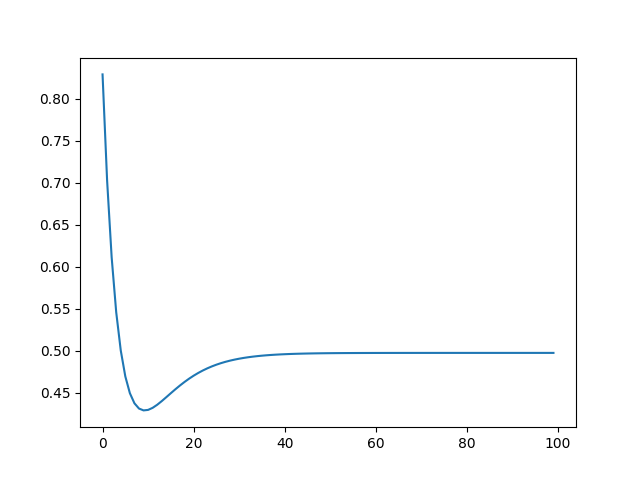
\includegraphics{925.png}
\end{center}

 With this particular model converegence can further be determined by the target function to the model which in this case gave 7 digits of accuracy after 100 iterations 
($\theta_{real} = 0.48810335753783995$, $\theta_{ predicted} = 0.48810336800164367$).  From the graph it is also clear that almost as good an approximation would have been obtained
with half as many (or fewer) iterations. 
 
Running 30 tests for each number of variables from 2 to 11 and analyzing the convergence of $\theta_{1}$ (the algorithm is symmetric in $\theta_{i}$ so there is no harm in this) leads to the following estimates for the number of iterations by which we expect convegence to begin. 

\begin{tabular} {cc}
\# of vars & estimate \\
2 & does not converge with this alpha\\
3 &  10 \\
4 &  12 \\
5 &  15 \\
6 &  20 \\
7 &  25 \\
8 & 30 \\
9 & 35 \\
10 & 40\\
11 & 40

\end{tabular} 

These are, of course rough estimates, based on a small sample, but they appear to indicate a pretty linear growth and lead to the initial hypothesis to look for convergence after $4n$ iterations where $n$ is the number of variables. 

Another look at the graph shows that the distance between the local min on the curve and the value to which it converges is less than .1.  This was true for all 270 models that converged,
so we expect that if all points start to tend to be within .1 of eachother the curve is on its way to convergence.  In this case $\alpha$ is $.01$ so our bound of $.1$ can be though of as 
$10\alpha$.  We give a silightly more conservative initial estimate: that we can choose $\epsilon$ to be 5 $\alpha$. 

Putting it together we conjecture that the method of gradient descent has converged on iteration $k$ if 
$$\forall\ k - 4n \leq  j,m \leq k, \hspace{.2in} 
|\theta_{i_{j}} - \theta_{i_{m}}| < 5\alpha$$  

\subsection{The Cost of Implementing the Condition}
To implement this condition it will at worst be necessary to keep a matrix of the n+1 values of each coefficient over 4n iterations and checking them which means the cost of 
implementing the proceduce is on the order $n^2$ checks per iteration in particular this is constant with respect to the size of the training set. Each iteration of the gradient descent method requires computations at least on the order of $n$ times the number of data points in the training set, so unless the number of variables is greater than the number of data points (which probably wouldn't converge anyway), implementing the test required above will lower the computational cost of running the algorithm (significantly). 

\subsection{Empirical Data}
To gauge the effectiveness of this method to detect convergence, 30 more simulations for each number of variables from 3 to 11 were performed, and the result of the Gradient Descent after 100 iterations and after the Cauchy cutoff were compared. On average the theta from the Cauchy estimate agreed with the real value of the coefficient to within .0001 for low numbers of variables and .001 for larger.  The following table gives an idea of the averge number of computations for caucy convergence and to what accuracy: 

\begin{tabular} {ccc}
\# of vars & average iterations to converge & Cauchy accuracy\\
3 &  15 & .0001 \\
4 &  21  & .001 \\
5 &  27 & .001 \\
6 &  33 & .001 \\
7 &  38 & .001 \\
8 & 45 & .001 \\
9 & 49 & .001\\
10 & 55 & .001\\
11 & 65 & .001

\end{tabular} 

The accuracy of the coefficients from 100 iterations continued to be within .00001 at 11 variables.  So there was a loss of a couple places of accuracy, but about a 33\% savings in computation.  Probably not a bad trade off in most situations.  

The entirety of the data referred to above as well as the source code used to generate it and a copy of this paper can be found on \href{ https://github.com/likes2addfunctions/CodeSamples/tree/master/GDCauchyMethod }{ GitHub} .

\subsection{The method of max $DJ$}
Recall that the method of gradient descent produces a new hypothesis by taking 
$$\Theta_{\mbox{new}} = \Theta - \alpha DJ.$$
Formally one may write 
$\Theta_{j+1} = \Theta_{j} - \alpha DJ_{j}$ 
and $\theta_{i_{j}} - \theta_{i_{j+1}} = \alpha DJ_{i_{j}}$. 
 Furthermore,
$$|\theta_{i_{j}} - \theta_{i_{m}}| = | \alpha \sum_{p=j}^{m-1}  DJ_{i_{p}}| \leq$$
$$\alpha \sum_{p=j}^{m-1}  |DJ_{i_{p}}| \leq \alpha \sum_{p=j}^{m-1} \max_{i \in \{0, \dots , n\}} |DJ_{i_{p}}|. $$

Then we can reformulate the satement in section 3 and suspect convergence if 
$$\alpha \sum_{p=k}^{k+4n-1} \max_{i \in \{0, \dots , n\}} |DJ_{i_{p}}| < 5\alpha$$
 A more elegant refinement of the conjecture is that the method of gradient descent on $n$ variables has converged on iteration $k$ if 

$$\sum_{p=k-2n}^{k} \left( \max_{i \in \{0, \dots , n\}} |DJ_{i_{p}}| \right)\  <\ 1 $$  

\subsubsection{Computational savings of max $DJ$ method}
To implement the max $DJ$ method the algorithm must perform at most $n$ checks on the $DJ$ vector to obain the max and then a set amount of operations to maintain a list of the most recent $DJ$s and replace values in the current sum.  In particular this is linear with respect to the number of variables and still constant with respect to the size of the data set. 

\section{Applying the Method to neural networks} 
The effective of this method on gradient descent begs the question of wheather it can be applied to more complicated learning techniques. Happily the answer is yes, with a slight modifaction.  The major complication comes from the fact that linear models produce convex sets over which a minimum must be obtained, while more general methods, such as neural networks, produce with local minimums.  One of the challenges in maximizing the effectiveness of a learning method is to avoid gettting caught in a local minimum. In order to avoid this, the idea is to perturb the values of the weights when a minimum is obtained. One way of doing this that has been suggested is to as a bit of randomness to each iteration in hopes of "jiggling" your way out of a shallow local min.  This issue with this is how much to jiggle, too much and you fly out of the local min, not enough and you never escape.  The method of max DJ, when applied to the weights of the neural network can be used to instead smoothly (and thus more quickly) descend upon a local minimum and then make an informed bump. 


\begin{figure}
 \begin{center}
\includegraphics[scale=.3]{fcsml1.png}
\end{center}
\caption{Getting Stuck at a Local Minimum}
\end{figure}

\subsection{Neural Networks}
There are many different types of neural networks, cost, functions, and methods for training them, but all neural netowrks consisst of layers of nodes, with each node having it's own weight. Each weight can change on each training example, so in principal, each weight should carry 3 indices : $w_{k}{lj}$ where k is the iteration number, $l$ is the layer and $j$ the position within the layer.   In a similar fashion to the convergence of gradient descent, the convergence of a neural network essentially amounts to the stabilization of these weights.  One major difference that weights are updated after each training examples instead of an entire epoch.  As such, the change in a weight after an iteration is no longer dictated by the graditent of the cost function, but computed through different methods (which depend on the specific type of neural network being implemented. 

\subsection{Tweaking Max DJ for NNs}
In some ways, the method needs very little tweaking: We can still make a vector $DJ_{k}$ whose components are the changes in each weight after iteration $k$ and we can still consider the sum 
$$\sum_{p=k-2n}^{k} \left( \max_{i \in \{0, \dots , n\}} |DJ_{i_{p}}| \right)\ $$
where $n$ is the total number of weights. When this sum is small enough the algorithm has found a local minimum. 

As mentioned above the interesting part is to avoid getting caught in a local minimum.  When a local minimum is found we will store that set of weights as a hypothesis $h$ and then vary the weights appropriately in hopes of climbing out of a local minimum.  The idea move away from the direction which has been changing most quickly in the weight space.  So suppose that we have decided that $\sum_{p=k-2n}^{k} \left( \max_{i \in \{0, \dots , n\}} |DJ_{i_{p}}| \right)\ $ is small enough and we have reached a local minimum, $h_{t}$, we can construct the vector
$DJ_{h_{t}} = \sum_{p=k-2n}^{k} DJ_{p}$.  The coordinates of this vector are simply the sum in the changes of each weight.  We can now perturb $h$ by changing weight $w_{i}$ by $ce^{-|DJ_{p}^{i}}$ where $c$ is an appropriately chosen constant.  In this way we move away from the direction in which we were decending most steeply and are more likely to "get over the hill" from the new starting point from which to decend we have created $H_{0_{t}} = h_{t} - e^{DJ_{h_{t}}}$. If we find $T$ such that $h_{T}  = h_{T+1}$ then we have generated a possible set of best hypotheses $h_{1}, h_{2}, ... h_{T}$ which can then be tested against validation data to determine which is most effective. It should be noted that this list may not be exhaustive of all local minimums and it will probably still be valueable to reiterate this whole process from a different initial hypothesis. 


\section{Proposals for Future Research}
\begin{itemize}
\item Refine Estimate of computation savings 

\item Provide analytic justification/refinement of estimates for $k_{0}$ and $\epsilon$. 

\item Make precise connection between size of alpha, intensity of randomness, and convergence

\end{itemize}







\end{document}
